\chapter{嵌入式硬件平台简介及内核运行}
\section{基于嵌入式硬件的操作系统开发流程}
随着计算机处理器制造技术的日新月异和集成电路的蓬勃发展,小小的芯片上就可以搭载一个强大的处理器,这也就为嵌入式系统营造了一片良好的土壤,为嵌入式开发创造了一片蓝海。日常生活中,嵌入式系统无处不在,我们使用的手机,平板电脑,空调,冰箱等各种各样的物件中,都存在嵌入式系统的影子。

嵌入式系统的开发与传统的PC程序开发是不用的。其设计了硬件和软件的开发,是一个协同工作的统一体。

那么什么是嵌入式系统?

嵌入式系统的英文名称是Embedded System。embedded意为嵌入...之中的,system意为系统。嵌入式系统有一些显著的特点,它的形式多样、体积比较小,可以灵活地适应各种设备的需求,能够根据用户需求灵活地裁剪软硬件模块。

嵌入式操作系统是计算机发展的一个方向,是一个体积小型化,功能多样化的方向,而另一个方向则是体积大型化,处理能力超强的大型计算机。计算机大型化适用于那些需要进行大量数据存储和大量数据处理的环境中,例如银行需要的是计算机的处理能力和稳定性,计算机的功耗和占用空间反而是其次需要考虑的。计算机小型化适用于响应时间和数据吞吐要求不高,但对功耗和空间占用有要求的场景,像是手机,PC电脑,电冰箱,空调等设备。

嵌入式操作系统种类繁多,按照系统硬件的核心处理器来区分,可以分为嵌入式微控制器和嵌入式微处理器。嵌入式微控制器就是传统意义上的单片机。单片机就是把一个计算机的主要功能集成到了一个芯片上,其通常包含了运算处理单元、ARM、flash存储器,以及一些IO接口。嵌入式微处理器与单片机相比,其处理器的处理能力更强,目前主流的嵌入式未处理为32位,单片机多是8位和16位。嵌入式微处理器在一个芯片上集成了复杂的功能,其有运算单元,指令存储器,数据存储器,缓冲区,总线,一些IO接口。在这样一个功能完善的处理器上,就可以搭载操作系统,帮助嵌入式开发。下图为嵌入式微处理器的基本结构。

\begin{figure}[H]
	\centering
	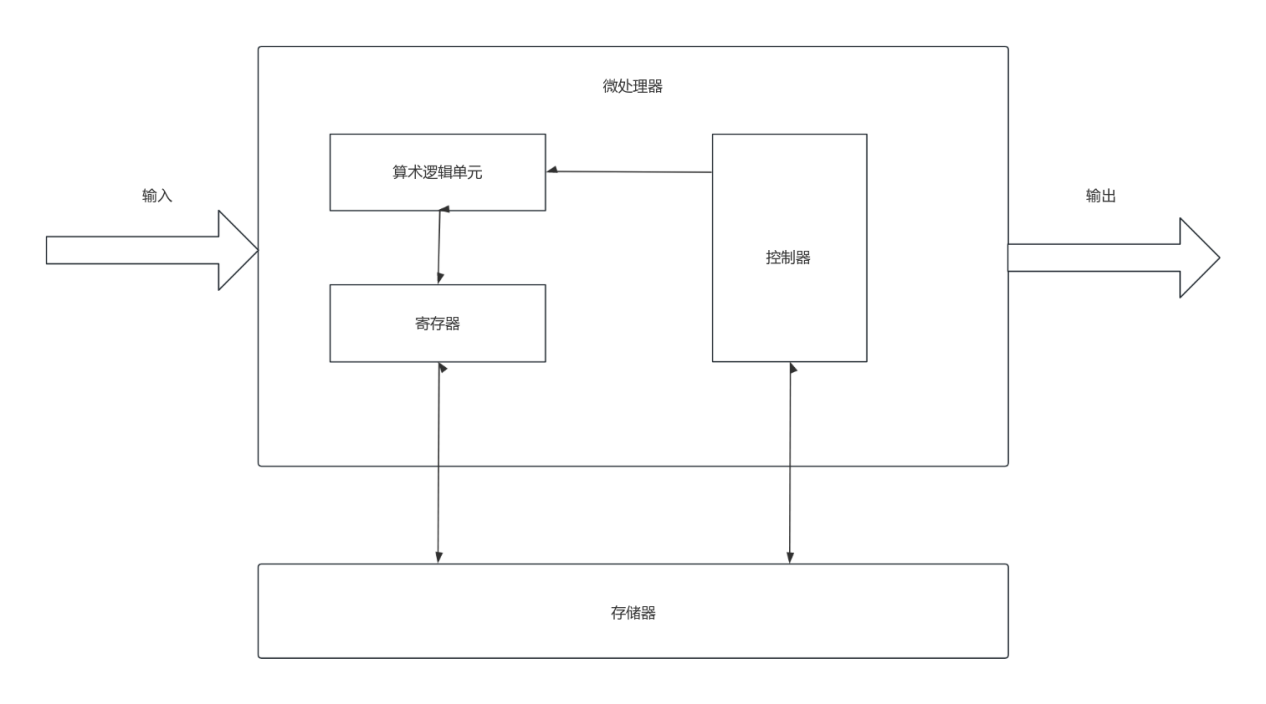
\includegraphics{figures/08-01-嵌入式微处理器基本结构.png}
	\caption{嵌入式微处理器的基本结构}
\end{figure}

嵌入式系统按层次来分,与传统pc一样,仍然分为硬件和软件层,硬件层包括嵌入式微处理器和各种外部设备,根据应用需求的不同,各种外部设备又各不相同;软件层又可以分为操作系统和应用软件两层,操作系统作为软硬件接口,负责管理系统资源,这与传统pc是一样的,用户仍然与应用软件打交道,看不到下层。

一般情况下,我们在一台计算机上编写了代码,便直接用该计算机上的编译器,编译后的到可执行代码,程序便可以执行,像这样的情况,我们就称之为“本地编译”。然而,有的时候我们并不能本地编译,我们需要在一种平台上编译出能运行在体系结构不同的另一种平台上能够运行的程序,也就是需要“交叉编译”。嵌入式开发过程中,目的平台常常还没有操作系统,谈不上运行编译器,平台运行至少需要两个东西,bootloader(启动引导代码)以及操作系统核心。这种情况下,我们只能求助于交叉编译。

在一个平台上编译成功后,我们便可以将操作系统烧写入开发板(目的平台)中,但在烧写之前,我们还涉及到了一个计算机与开发板的通信问题,这也就涉及到了串口这个概念,我们通过串口,实现计算机与外部设备的通信,来解决把操作系统烧写入开发板的问题。

\subsection{串口简介}

\subsubsection{什么是串口}

串口是串行接口(Serial Port)的简称,是一种常用的计算机接口。由于连线少、通信控制简单而得到广泛的使用。串口有几种标准,常见的一种称为 RS232 接口的标准是在1970年由美国电子工业协会(EIA)和几家计算机厂商共同制定的。RS232标准应用广泛,其全称是“数据终端设备(DTE)和数据通讯设备(DCE)串行二进制数据交换接口”,该标准定义了串口的电气接口特性和各种信号电平等。


标准串口协议支持的最高数据传输率是115Kbps。一些改进的串口控制器支持更高甚至460Kbps的数据传输率,如增强型串口ESP(Enhanced Serial Port)和超级增强型串口Super ESP。


RS232 串口使用D型数据接口,最初有9针和25针两种连接方式。随着计算机技术的不断进步,25针的串口连接方式已经被淘汰,目前所有的RS232串口都使用9针连接方式。

\subsubsection{串口工作原理}

串口通过直接连接在两台设备之间的线发送和接收数据,两台设备通信最少需要三根线(发送数据、接收数据和接地)才可以通信。以最常见的RS232串口为例,通信距离较近时(<12m),可以用电缆线直接连接标准RS232端口。如果传输距离远,可以通过调制解调器(MODEM)传输。因为串口设备工作频率低且容易受到干扰,远距离传输会造成数据丢失。

\begin{table}[!ht]
	\centering
	\begin{tabular}{|c|c|c|}
		\hline
		\textbf{针号} & \textbf{功能说明} & \textbf{缩写} \\
		\hline
		1 & 数据载波检测 & DCD  \\
		2 & 接收数据 & RXD  \\
		3 & 发送数据 & TXD \\
		4 & 数据终端准备 & DTR \\
		5 & 信号地 & GND \\
		6 & 数据设备准备好 & DSR \\
		7 & 请求发送 & RTS \\
		8 & 清除发送 & CTS \\
		9 & 振铃指示 & BELL \\
		\hline
	\end{tabular}
	\caption{DB9接口的RS232 串口数据线定义}
	\label{DB9接口的RS232 串口数据线定义}
\end{table}

表 \ref{DB9接口的RS232 串口数据线定义}是常见的9针接口串口各条线定义,RS232标准的串口不仅提供了数据发送和接收的功能,同时可以进行数据流控制。对于普通应用来说,连接好两个数据线和地线就可以通信。

\subsubsection{Windows系统下的串口工具}

MobaXterm 又名 MobaXVT,是一款增强型终端、X 服务器和 Unix 命令集(GNU/ Cygwin)工具箱。可以开启多个终端视窗,以最新的 X 服务器为基础的 X.Org,可以轻松地来试用 Unix/Linux 上的 GNU Unix 命令。这样一来,我们可以不用安装虚拟机来试用虚拟环境,然后只要通过 MobaXterm 就可以使用大多数的 linux 命令。MobaXterm 还有很强的扩展能力,可以集成插件来运行 Emacs、Fontforge、Gcc, G++ and development tools、MPlayer、Perl、Curl、Corkscrew、 Tcl / Tk / Expect、 Screen、 Png2Ico 、 NEdit  Midnight Commander 等程序。


MobaXterm的下载较为简单,进入官网直接下载即可。需要注意的是MobaXterm 分免费家庭版和收费专业版:
\begin{itemize}
	\item 家庭版(Home):家庭版又分便捷版和安装版。便捷版不需要安装,下载压缩包后解压即可使用。安装版则需一步步安装后才能使用。
	\item 专业版(Professional):专业版会在 Session数、SSH tunnels 数和其他一些定制化配置进行限制。
\end{itemize}

MobaXterm的界面结构为:
\begin{itemize}
	\item 主页:打开MobaXterm后,绝大部分内容会被主页占据,主页有快捷按钮“start local terminal”以及最近的Session记录,可以方便打开终端,进行命令行操作。
	\item 菜单栏:MobaXterm的菜单栏如下,分为menu bar和buttons bar两行。用户可通过menu bar设置MobaXterm。buttons bar则为用户提供了一系列功能,如用户可通过Session启动远程会话,选择创建 SSH、Telnet、Rlogin、RDP、VNC、XDMCP、FTP、SFTP 或串行会话。开始的每个会话都会自动保存并显示在左侧边栏中。
	\item 侧边栏:侧边栏分为三个视图,分别为Sessions,Tools,Macros。Sessions负责管理使用过的Session配置,可以在任意Session选项上右击进行编辑。Tools分为四部分Terminal games、System、Office、NetWork的工具集合。使用非常的方便。Macros可以录制操作过程,下次使用时直接回放即可。
\end{itemize}

\begin{figure}[h]
	\centering
	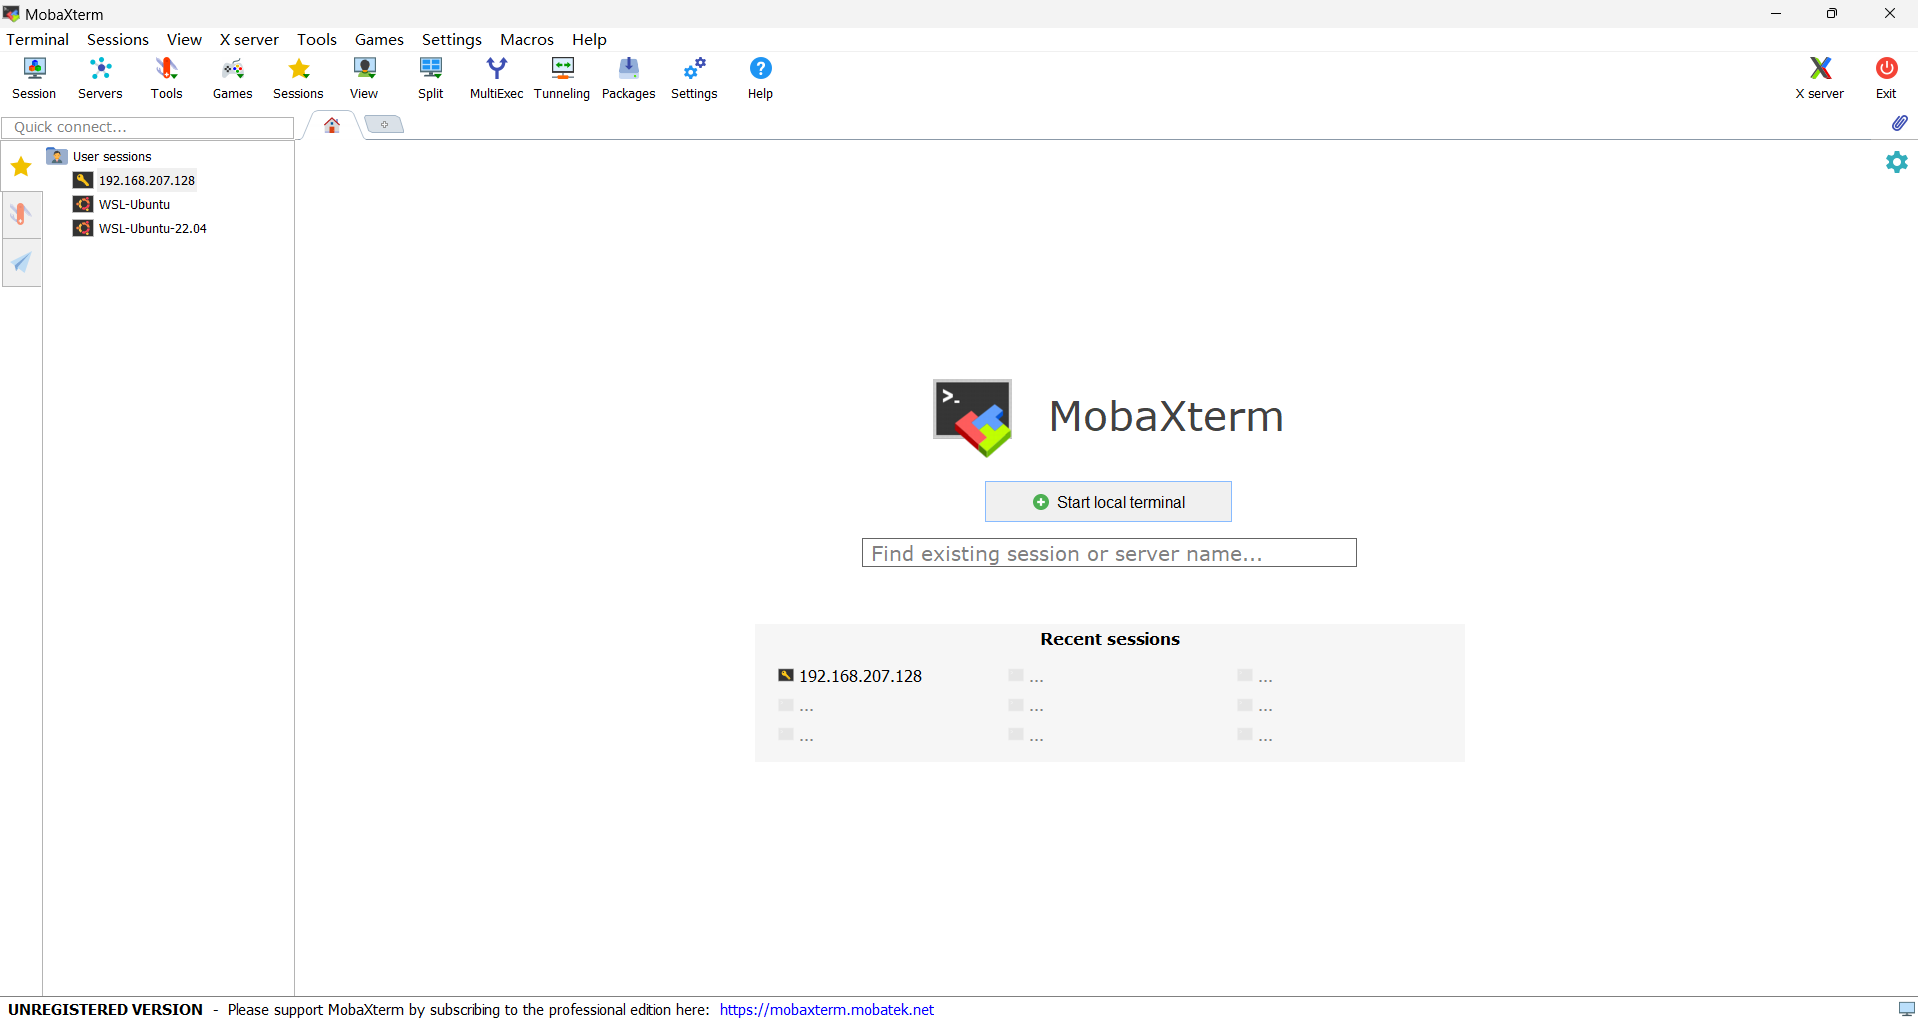
\includegraphics[width=0.6\textwidth]{figures/08-01-mobaXterm界面.png}
	\caption{mobaXterm界面}
	\label{mobaXterm界面}
\end{figure}


MobaXterm是一款功能强大的综合性工具,支持SSH、RDP、FTP、Serial等多种通信协议。在本节中,我们将重点介绍其支持的Serial协议功能。MobaXterm可用作串口终端,与串口调试助手等工具相比,它提供了更强大的功能。在使用串口调试助手等工具时,虽然可以用于打印调试信息,但无法实现终端使用,即不能输入命令。


在MobaXterm中,通过点击"Session",选择"Serial",打开串口设置窗口。首先,选择要配置的串口号,并使用串口线将开发板连接到计算机上。然后,设置波特率,MobaXterm软件能够自动识别串口,用户只需从下拉菜单中选择相应的波特率。此外,还需进行其他串口功能的设置。点击"Advanced Serial settings"选项卡,可配置串口的其他功能,包括串口号、数据位、停止位、奇偶校验和硬件流控等。若需配置与终端相关的功能,则可点击"Terminal settings",进行相关设置,如终端字体以及字体大小等。完成设置后,点击窗口下方的"OK"按钮即可。

\subsubsection{Linux系统下的串口工具}

串口是嵌入式开发使用最多的通信方式。Linux系统提供了一个串口工具minicom,可以完成复杂的串口通信工作。若将minicom移植到板卡上,我们就可以借助minicom对串口进行读写操作。


本节介绍 minicom的使用。首先是安装 minicom,在 Ubuntu Linux 系统 shell 下输入“sudo apt-get install minicom”,按回车键后即可安装minicom 软件。软件安装好后,第一次使用之前需要配置minicom。

\begin{enumerate}
	\item 在shell中输入 sudo minicom-s,出现 minicom配置界面,下图 \ref{minicom配置界面}所示。minicom配置菜单在屏幕中央,每个菜单项都包括了一组配置。
	\begin{figure}[h]
		\centering
		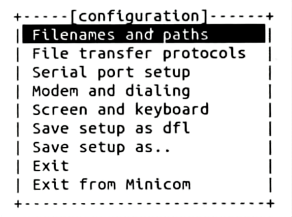
\includegraphics[width=0.4\textwidth]{figures/08-01-minicom配置界面.png}
		\caption{minicom配置界面}
		\label{minicom配置界面}
	\end{figure}

	\item 用光标键移动高亮条到 Serial Port setup菜单项,按回车键后进入串口参数配置界面,如下图 \ref{minicom配置端口界面}所示。串口配置界面列出了串口的配置,每个配置前都有一个英文字母,代表进入配置项的快捷键。首先配置端口,输入小写字母a,光标移动到了/dev/tty8字符串最后,并且进入
	到编辑模式。以笔者机器为例,修改为/dev/tty0,代表连接到系统的第一个串口。
	\begin{figure}[h]
		\centering
		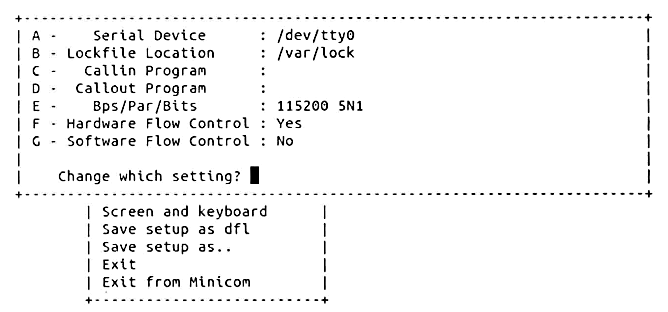
\includegraphics[width=0.6\textwidth]{figures/08-01-minicom配置端口界面.png}
		\caption{minicom配置端口界面}
		\label{minicom配置端口界面}
	\end{figure}

	\item 配置好串口设备后按回车键,保存参数并且回到提示界面。输入小写字母e,进入串口参数配置界面,如下图 \ref{minicom配置串口参数}所示。串口参数界面可以配置串口波特率、数据位、停止位等信息。一般只需要配置波特率,如在笔者机器上需要配置波特率是38400,输入小写字母d,屏幕上方current字符串后的波特率改变为38400。
	\begin{figure}[h]
		\centering
		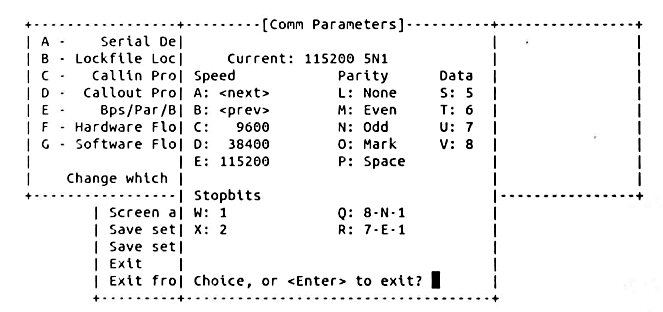
\includegraphics[width=0.6\textwidth]{figures/08-01-minicom配置串口参数.png}
		\caption{minicom配置串口参数}
		\label{minicom配置串口参数}
	\end{figure}

	\item 设置好波特率后按回车键,保存退出,回到串口配置界面,如下图 \ref{minicom配置端口结束}所示。串口被设置为tty0,波特率是38400,其他配置使用默认设置。如果保存配置,直接按回车键退出。选择Save setup as dfl选项后按回车键,配置信息被保存为默认配置文件,下次启动的时候会自动加载。保存默认配置后,选择Exit选项后按回车键,退出配置界面,minicom自动进入终端界面。在终端界面会自动连接到串口,如果串口没有连接任何设备,屏幕右下角的状态提示为Offline。
	\begin{figure}[h]
		\centering
		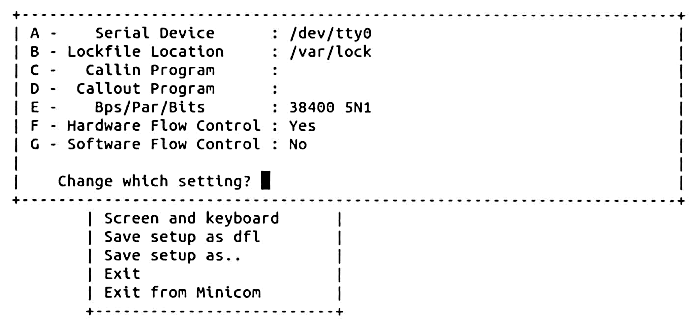
\includegraphics[width=0.6\textwidth]{figures/08-01-minicom配置端口结束.png}
		\caption{minicom配置端口结束}
		\label{minicom配置端口结束}
	\end{figure}

	\item 退出 minicom,使用Ctrl+a键,然后输入字母z,出现minicom的命令菜单,如下图 \ref{minicom命令界面}所示。
	\begin{figure}[h]
		\centering
		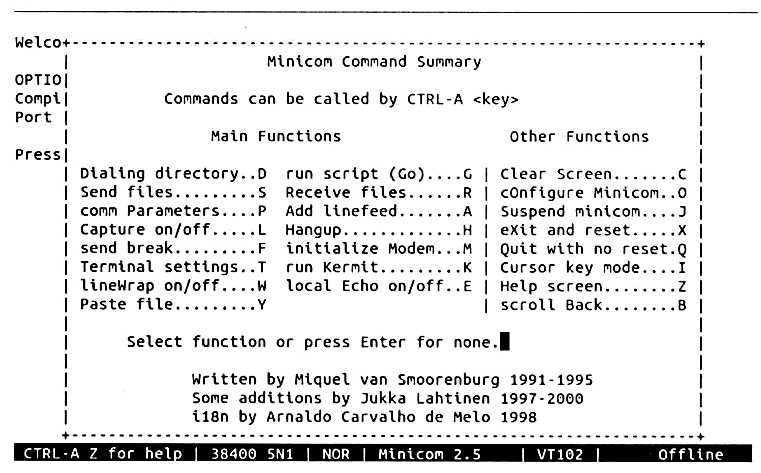
\includegraphics[width=0.6\textwidth]{figures/08-01-minicom命令界面.png}
		\caption{minicom命令界面}
		\label{minicom命令界面}
	\end{figure}
\end{enumerate}



Minicom 提供了丰富的功能,是 Linux 中串口通信和远程管理的重要工具:

\begin{itemize}
	\item 调试和配置串口设备: Minicom 可以连接和调试各种串口设备,如调制解调器、路由器、交换机等。用户可以通过 Minicom 查看设备的输出信息,发送指令进行配置和调试。

	\item 远程终端连接: Minicom 可以作为一个终端仿真器,用于远程连接到其他计算机或设备。通过串口连接,用户可以在本地计算机上操作远程设备,进行远程管理和维护。

	\item 数据传输和文件传输: Minicom 支持通过串口进行数据传输,可用于传输文件、备份数据等。用户可以通过 Minicom 将文件发送到远程设备或从远程设备接收文件。

	\item 系统调试和故障排查: Minicom 可用于调试和排查系统故障。通过串口连接到系统控制台,用户可以查看系统的启动信息、错误日志等,帮助定位和解决问题。

	\item 嵌入式开发和调试: 对于嵌入式系统开发者来说,Minicom 是一个重要的工具。它可用于与嵌入式设备进行通信,进行程序下载、调试和测试。
\end{itemize}

\subsection{U-Boot启动介绍}

Bootloader这个名词在嵌入式系统中应用广泛,中文意思可以理解为“启动加载器”。从字面意思来看,Bootloader就是在系统启动时运行的软件。由于系统启动涉及到硬件和软件的协同操作,因此Bootloader成为连接硬件和软件的关键系统软件之一。在我们的后续实验中,将会使用到一个广泛应用的开源Bootloader软件——U-Boot。

因此,在这一部分,我们将以U-Boot作为示例,介绍Bootloader的功能、工作流程、命令以及菜单选项的含义。接着,会详细讲解U-Boot中一种常用的启动方式——tftpboot,以及与tftpboot相关的tftp协议。最后,会分别探讨在Windows系统中使用软件Mobaxterm时tftp的位置以及如何配置使用,在Linux系统上如何下载安装tftp以及如何配置使用。

\subsubsection{U-Boot Bootloader的功能和工作流程}


    \textbf{ U-Boot的功能:}U-Boot作为一款强大的Bootloader软件,拥有多项关键功能。它管理系统启动过程、加载操作系统和初始化硬件,实现了引导加载、固件更新和系统维护。此外,U-Boot提供了丰富的命令集,允许用户与系统进行交互,进行存储器操作、网络传输以及系统配置,为嵌入式系统的开发和调试带来了灵活性和便利性。虽然U-Boot支持多种处理器和操作系统,但其在PowerPC系列处理器和Linux操作系统上的支持最为完善。它涵盖了许多嵌入式开发中常用的功能,例如查看、修改内存,以及通过网络下载操作系统镜像等,为开发者提供了良好的支持。U-Boot项目更新迅速,支持的目标板众多,是学习底层开发的极佳工具。
    
    \textbf{  U-Boot的工作流程:}大多数bootloader的启动流程都分为stage1和stage2两部分, U-Boot也不例外。依赖于CPU体系结构的代码(如设备初始化代码等)通常都放在stage1且可以用汇编语言来实现,而stage2则通常用C语言来实现,这样可以实现复杂的功能,而且有更好的可读性和移植性。
    
    \begin{figure}[h]
    	\centering
    	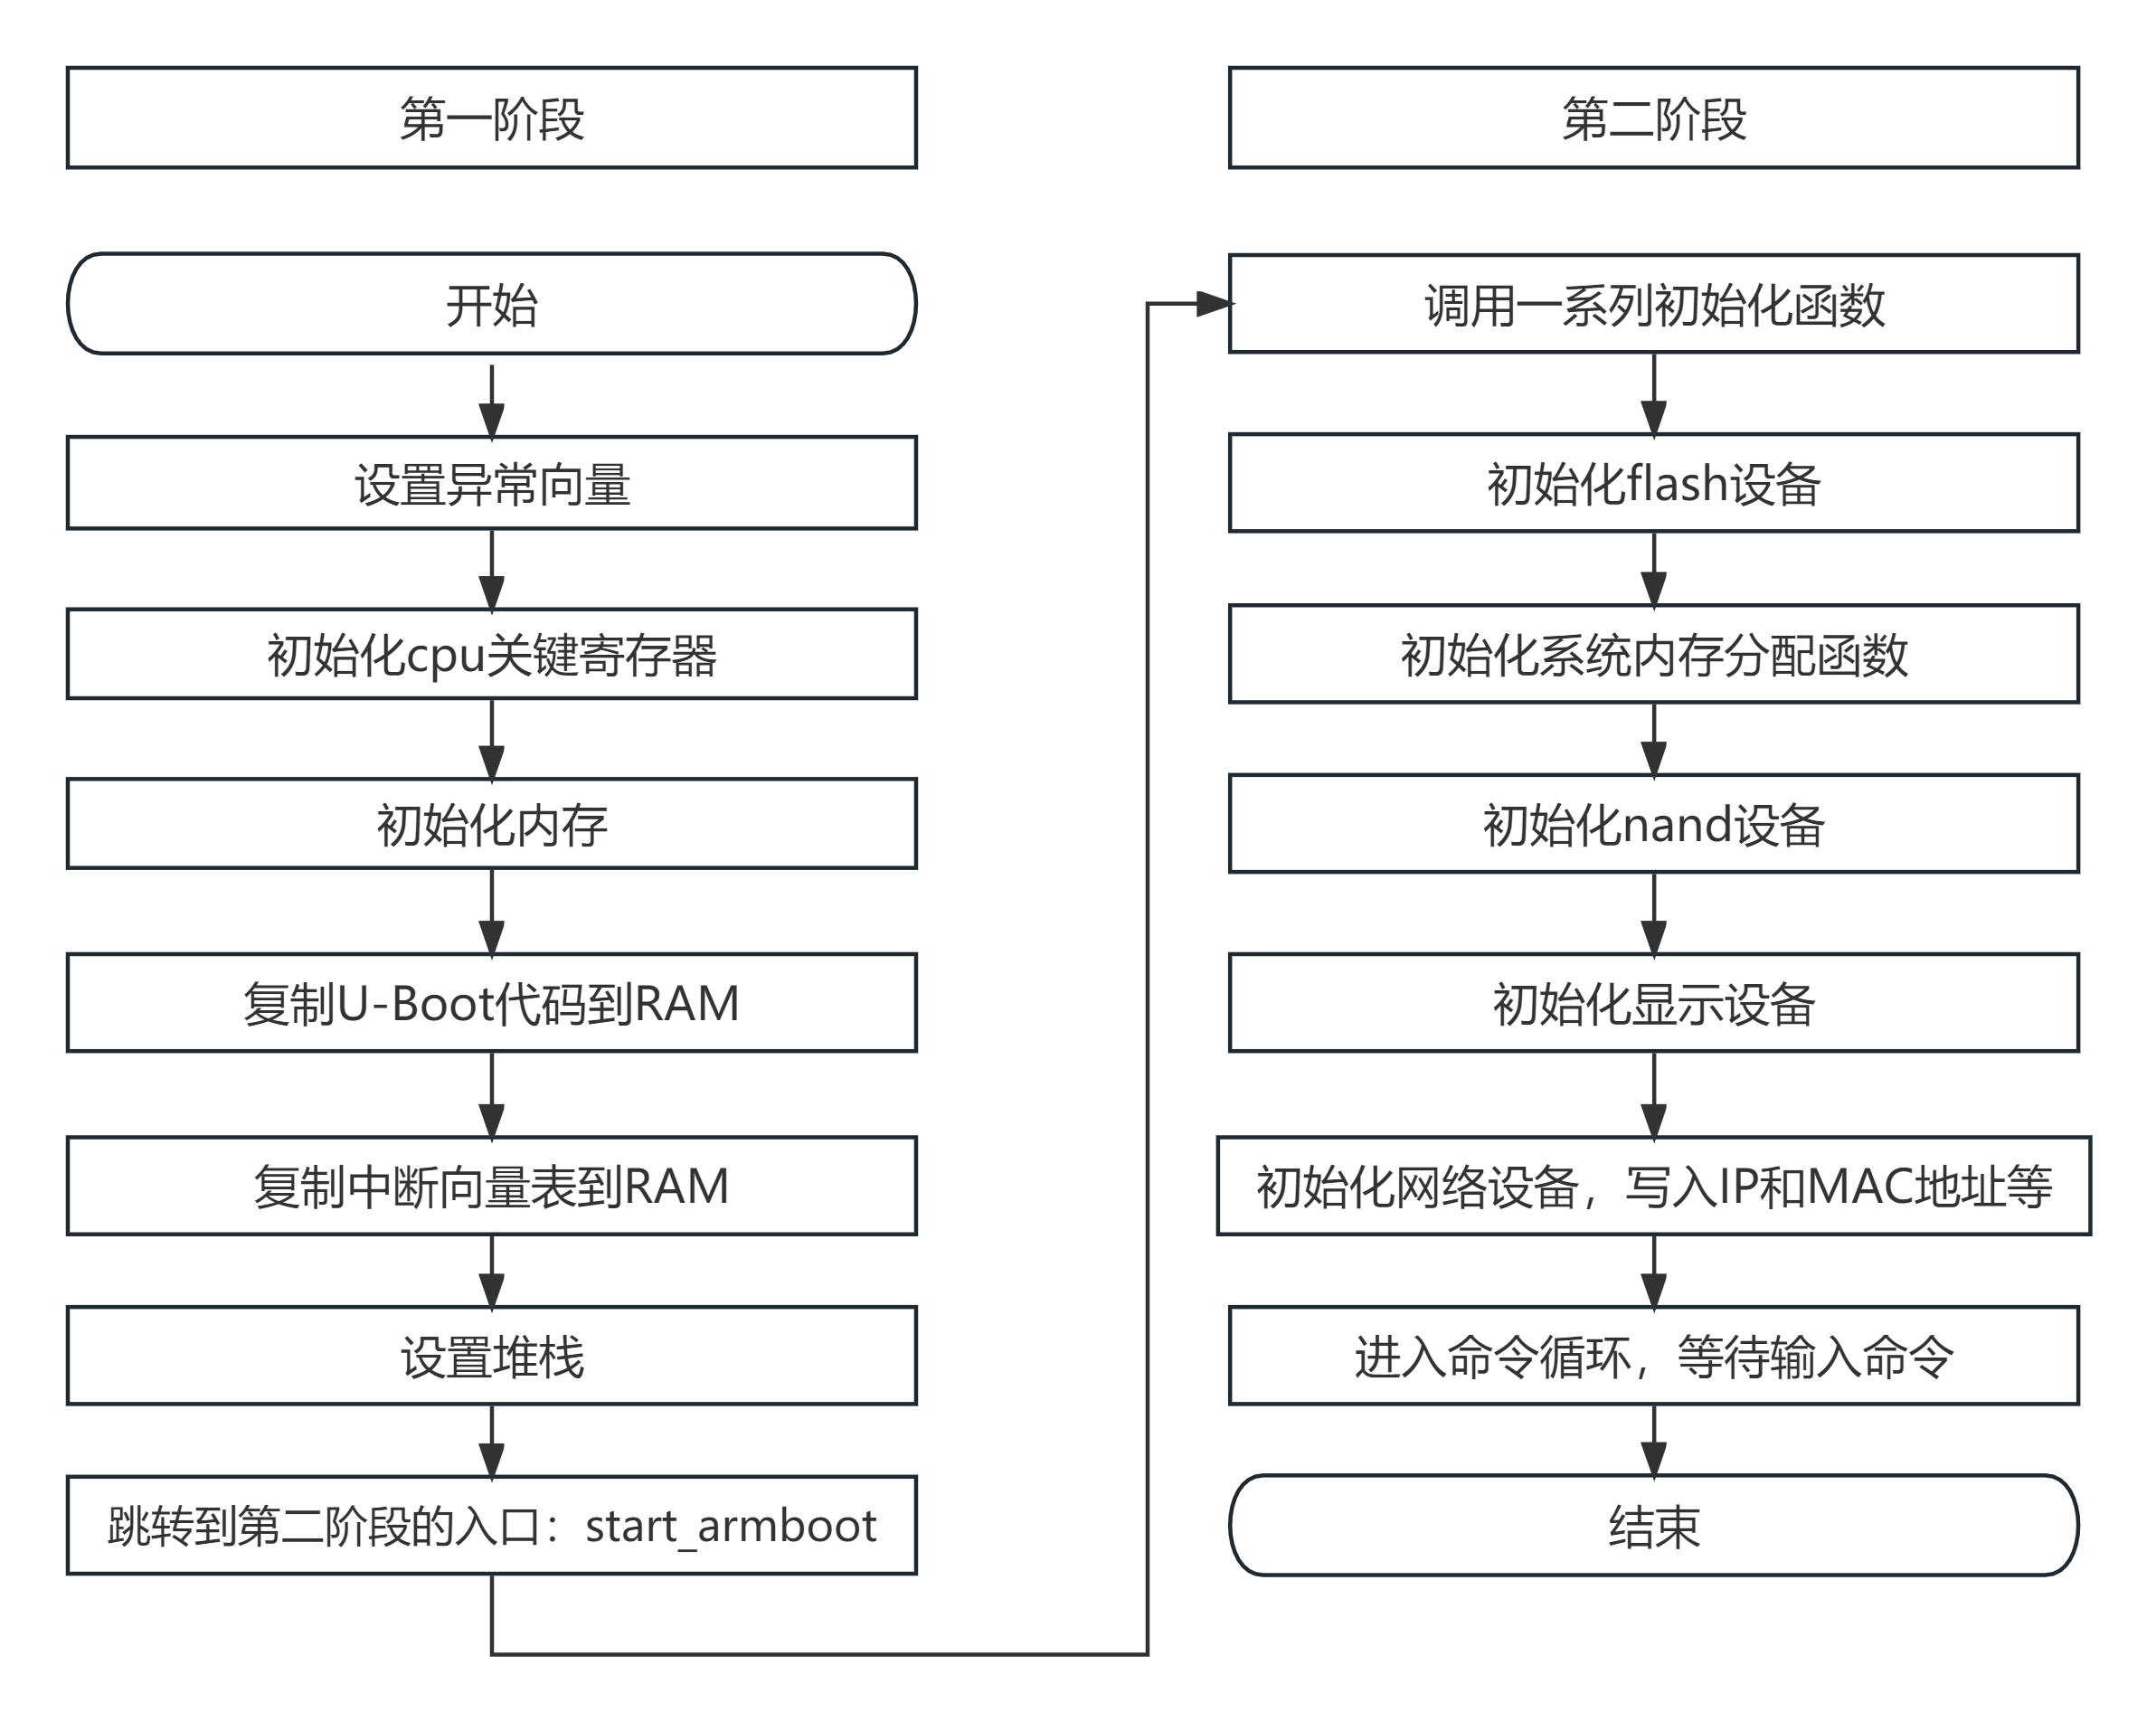
\includegraphics[width=0.8\textwidth]{figures/08-01-U-Boot的工作流程.png}
    	\caption{U-Boot的工作流程}
    	\label{U-Boot的工作流程}
    \end{figure}
    
    图8-8是U-Boot的整体工作流程。Stage1的代码都是与平台相关的,使用汇编语言编写占用空间小而且执行速度快。以ARM920为例,Stagel阶段主要是设置各模式程序异常向量表,初始化处理器相关的关键寄存器以及系统内存。Stage1负责建立Stagel阶段使用的堆栈和代码段,然后复制Stage2阶段的代码到内存。
    
    Stage2阶段一般包括初始化 Flash器件、检测系统内存映射、初始化网络设备、进入命令循环,接收用户从串口发送的命令然后进行相应的处理。Stage2使用C语言编写,用于加载操作系统内核,该阶段主要是board.c中的start\_armboot()函数实现。
    
    \textbf{ U-Boot的命令:}
    
   \begin{table}[!ht]
   	\centering
   	\begin{tabular}{|c|c|c|}
   		\hline
   		\textbf{类别} & \textbf{命令} & \textbf{功能说明} \\
   		\hline
   		信号查询 & bdinfo & 查看开发板信息 \\
   		信号查询 & printenv & 输出环境变量信息 \\
   		信号查询 & version & 查看U-Boot的版本号 \\
   		环境变量 & setenv & 设置或者修改环境变量的值 \\
   		环境变量 & saveenv & 保存修改后的环境变量 \\
   		内存操作 & md & 显示内存值\\
   		内存操作 & nm & 修改指定地址内存值,地址不会自增\\
   		内存操作 & mm & 修改指定地址内存值,地址会自增\\
   		内存操作 & mw & 使用一个指定的数据填充一段内存\\
   		内存操作 & cp & 用于将 DRAM 中的数据从一段内存拷贝到另一段内存中\\
   		内存操作 & cmp & 用于比较两段内存的数据是否相等\\
        网络操作 & ping & 检测网络的连通情况 \\
        网络操作 & dhcp & 从路由器获取 IP 地址 \\
        网络操作 & nfs & 通过nfs可以在计算机之间通过网络来分享资源 \\
        网络操作 & tftp & 使用TFTP协议通过网络下载东西到 DRAM 中\\
        EMMC和SD卡操作 & mmc info & 输出MMC设备信息 \\
        EMMC和SD卡操作 & mmc read & 读取MMC中的数据 \\
        EMMC和SD卡操作 & mmc wirte & 向MMC设备写入数据 \\
        EMMC和SD卡操作 & mmc dev & 切换MMC设备 \\
        FAT格式文件操作 & fatinfo & 查询指定MMC设置指定分区的文件系统信息 \\
        FAT格式文件操作 & fatls & 查询FAT格式设备的目录和文件信息 \\
        FAT格式文件操作 & fstype & 查看MMC设备某个分区的文件系统格式 \\
        FAT格式文件操作 & fatload & 命令用于将指定的文件读取到DRAM中 \\
        BOOT操作 & bootz & 自动zImage镜像文件\\
        BOOT操作 & bootm & 启动 uImage 镜像文件 \\
        BOOT操作 & boot& 读取环境变量bootcmd来启动Linux系统 \\
        其他常用操作 & reset & 复位重启 \\
        其他常用操作 & go & 跳到指定的地址处执行应用 \\
        其他常用操作 & run & 运行环境变量中定义的命令 \\
        其他常用操作 & mtest & 简单的内存读写测试命令 \\
   		\hline
   	\end{tabular}
   	\caption{U-Boot的命令表}
   	\label{U-Boot的命令表}
   \end{table}
   
     进入U-Boot的命令行模式以后输入“help”或者“?”,然后按下回车即可查看当前U-Boot所支持的命令。我们输入“help(或?)命令名”可以查看命令的详细用法。如图8-9所示,以“setenv”这个命令为例,我们输入如下命令即可查看“setenv”这个命令的用法:
     
     \begin{figure}[h]
     	\centering
     	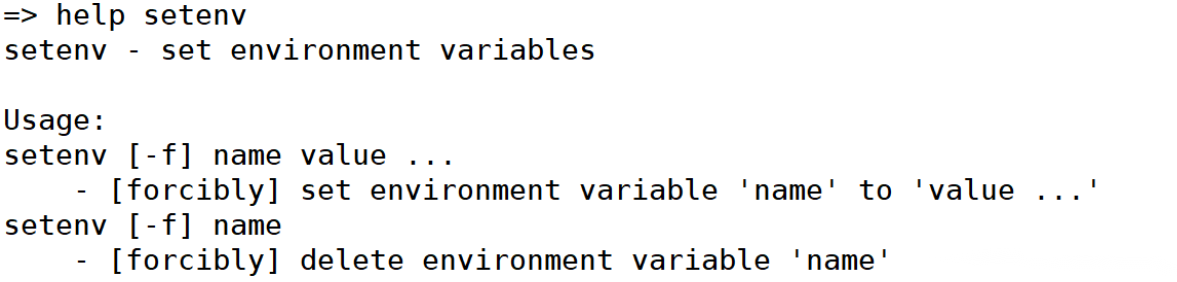
\includegraphics[width=0.8\textwidth]{figures/08-01-U-Boot命令行help使用实例.png}
     	\caption{U-Boot命令行help使用实例}
     	\label{U-Boot命令行help使用实例}
     \end{figure}
     
     \textbf{ U-Boot的菜单选项:}uboot菜单其实就是一个uboot中的命令,和其他的命令没有什么差别。 如图8-9所示,uboot启动时,如果进入uboot命令模式,先运行这个命令,就会打印出一个菜单界面。在uboot的命令模式,通过键入“menu”命令,同样可以调出这个界面。
     
    \begin{figure}[h]
    	\centering
    	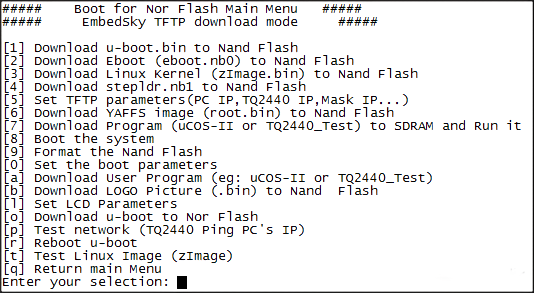
\includegraphics[width=0.8\textwidth]{figures/08-01-U-Boot的菜单选项.png}
    	\caption{U-Boot的菜单选项}
    	\label{U-Boot的菜单选项}
    \end{figure}
    
    这些U-Boot中的menu选项包含了各种针对系统启动和配置的操作,各选项具体功能分析如下:
    
   \textbf{[1]Download u-boot.bin to Nand Flash}: 用于将u-boot.bin文件下载到Nand Flash中,是更新或安装U-Boot引导程序的选项。
    
    \textbf{[2]Download Eboot (eboot.nb0) to Nand Flash}: 将Eboot(eboot.nb0)下载到Nand Flash,可能是针对特定引导程序或固件的更新。
    
   \textbf{[3]Download Linux Kernel(zImage.bin) to Nand Flash}: 将Linux内核(zImage.bin)下载到Nand Flash中,用于更新或安装Linux内核。
    
    \textbf{[4]Download stepldr.nb1 to Nand Flash}:将stepldr.nb1下载到Nand Flash,可能是针对特定引导程序或固件的更新。
    
    \textbf{[5]Set TFTP parameters (PCIP, TQ2440 IP, Mask IP...):} 用于设置TFTP参数,包括PC的IP地址、TQ2440的IP地址、子网掩码等。
    
    \textbf{[6]Download YAFFs image (root.bin) to Nand Flash}: 将YAFFs镜像(root.bin)下载到Nand Flash中,可能是针对系统根目录的更新或安装。
    
    \textbf{[7]Download Program (ucos-II or TQ2440_Test) to SDRAM and Run it}: 将程序(ucos-II或TQ2440_Test)下载到SDRAM并运行,用于测试或运行特定程序。
    
    \textbf{[8]Boot the system}: 启动系统,触发系统的启动过程。
    
    \textbf{[9]Format the Nand Flash}: 格式化Nand Flash,清除其上的数据并准备好用于存储。
    
    \textbf{[0]Set the boot parameters}: 设置引导参数,包括启动时的配置参数和选项。
    
    \textbf{[a]Download user's Program (eg: ucos-II or TQ2440_Test)}: 下载用户程序(例如ucos-II或TQ2440_Test),用于定制或特定应用程序的更新。
    
   \textbf{[b]Download Logo Picture (.bin) to Nand Flash}: 将Logo图片(.bin)下载到Nand Flash,可能是更新系统启动时显示的Logo。
    
    \textbf{[l]Set LCD Parameters}: 设置液晶显示屏(LCD)参数,包括分辨率、刷新率等。
    
    \textbf{[o]Download u-boot to Nor Flash}: 将U-Boot下载到Nor Flash,用于更新或安装U-Boot引导程序。
    
    \textbf{[p]Test network (TQ2440 Ping PC's IP)}: 对网络进行测试,Ping TQ2440到PC的IP地址,用于网络连接的调试和测试。
    
    \textbf{[r]Reboot u-boot}: 重启U-Boot引导程序。
    
    \textbf{[t]Test Linux image (zImage)}: 测试Linux镜像(zImage),可能是验证镜像完整性或针对错误的测试。
    
    \textbf{[q]Return main Menu}: 返回主菜单,退出当前菜单并回到主界面。
    
\subsubsection{tftpboot与tftp的关系及使用}

    tftpboot是U-Boot中一种常见的启动方式,它通过TFTP协议从网络中加载启动所需的镜像文件。
    
    TFTP(Trivial File Transfer Protocol,简单文件传输协议)是TCP/IP协议族中的一个用来在客户机与服务器之间进行简单文件传输的协议,提供不复杂、开销不大的文件传输服务,端口号为69。TFTP协议的设计目的主要是为了进行小文件传输,因此它不具备通常的FTP的许多功能,例如,它只能从文件服务器上获得或写入文件,不能列出目录,不进行认证。
    
    TFTP代码所占的内存较小,这对于较小的计算机或者某些特殊用途的设备来说是很重要的,这些设备不需要硬盘,只需要固化了TFTP、UDP和IP的小容量只读存储器即可。因此,随着嵌入式设备在网络设备中所占的比例的不断提升,TFTP协议被越来越广泛的使用。
    
    下面分别介绍windows系统以及linux系统中如何下载安装tftp和使用:
    
    \newpage
    
    \textbf{1.windows系统:}在windows系统中我们使用软件mobaxterm来支持tftp协议。
    
    首先在刚刚新建串口的界面点击“"Servers"window-->TFTP server”
    
    \begin{figure}[h]
    	\centering
    	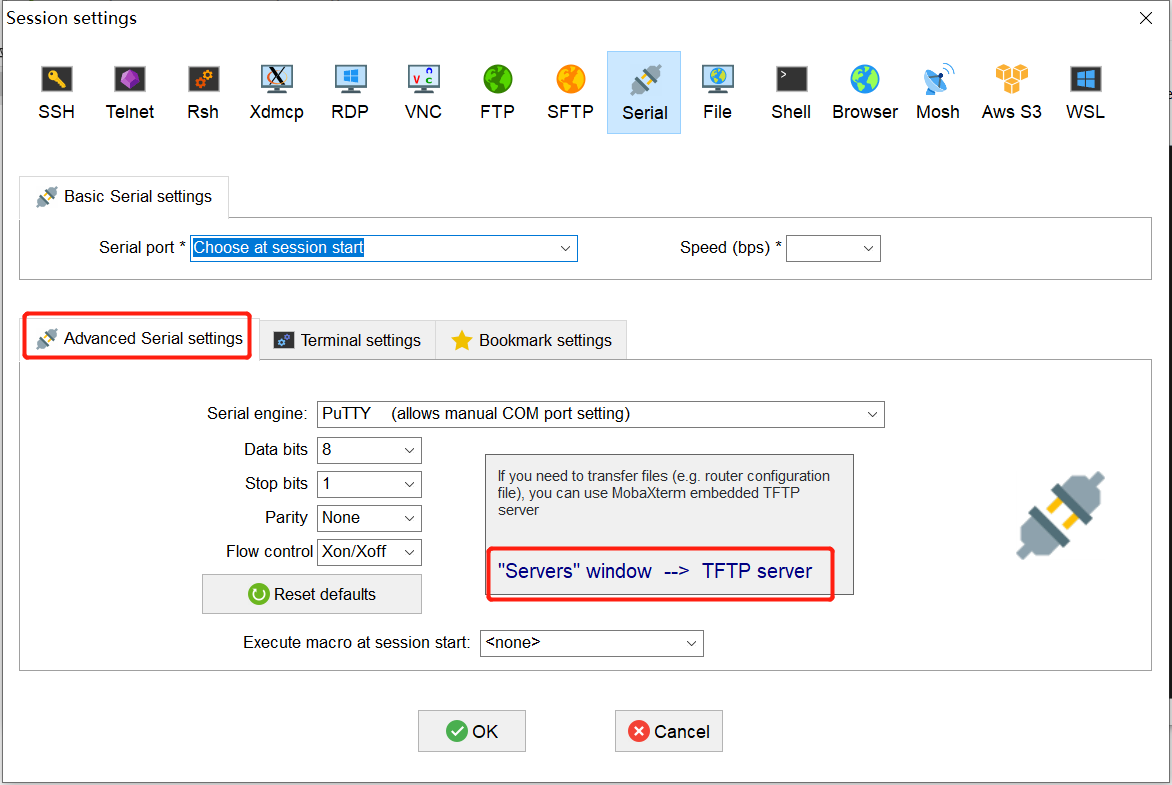
\includegraphics[width=0.8\textwidth]{figures/08-01-mobaXterm教程1.png}
    	\caption{mobaXterm教程1}
    	\label{mobaXterm教程1}
    \end{figure}
    
    然后在右方“Root directory”可以设置tftp服务器根地址,也就是开发板可以访问到的目录路径(包含编译出来的os.bin文件)。左上角点击运行按钮可以运行tftp服务:
    
    \begin{figure}[h]
    	\centering
    	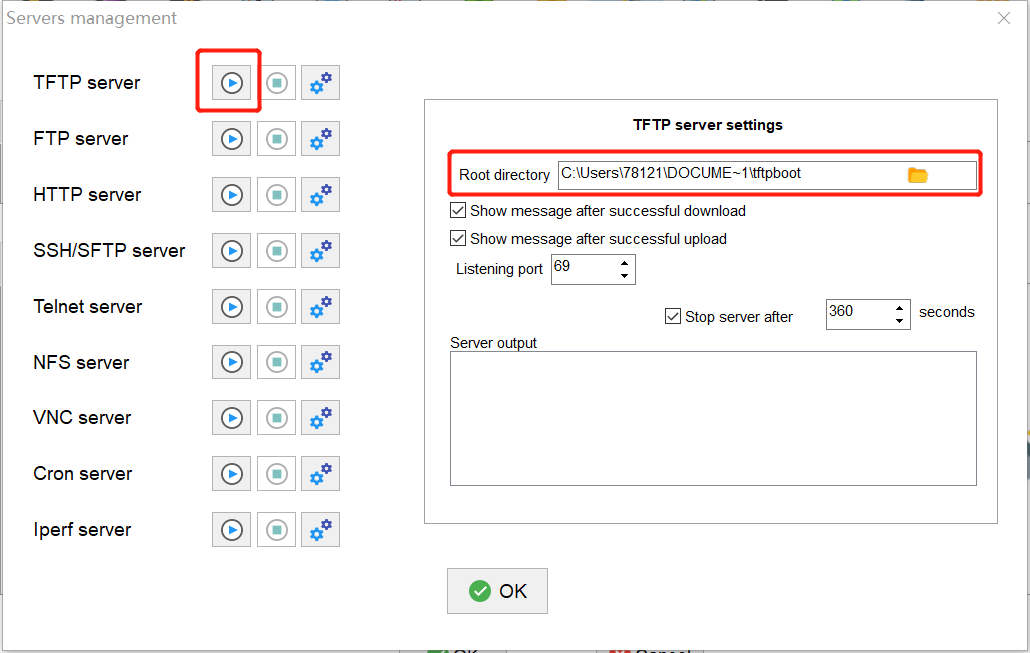
\includegraphics[width=0.8\textwidth]{figures/08-01-mobaXterm教程2.png}
    	\caption{mobaXterm教程2}
    	\label{mobaXterm教程2}
    \end{figure}
    
    运行按钮旁边的方框按钮为停止服务,右边显示“355”是服务剩余时间355秒,每次运行服务只可持续360秒,这是MobaXterm免费版的限制,服务到期后再通过同样的步骤启动服务。
   
    运行成功如下图:
    
    \begin{figure}[h]
    	\centering
    	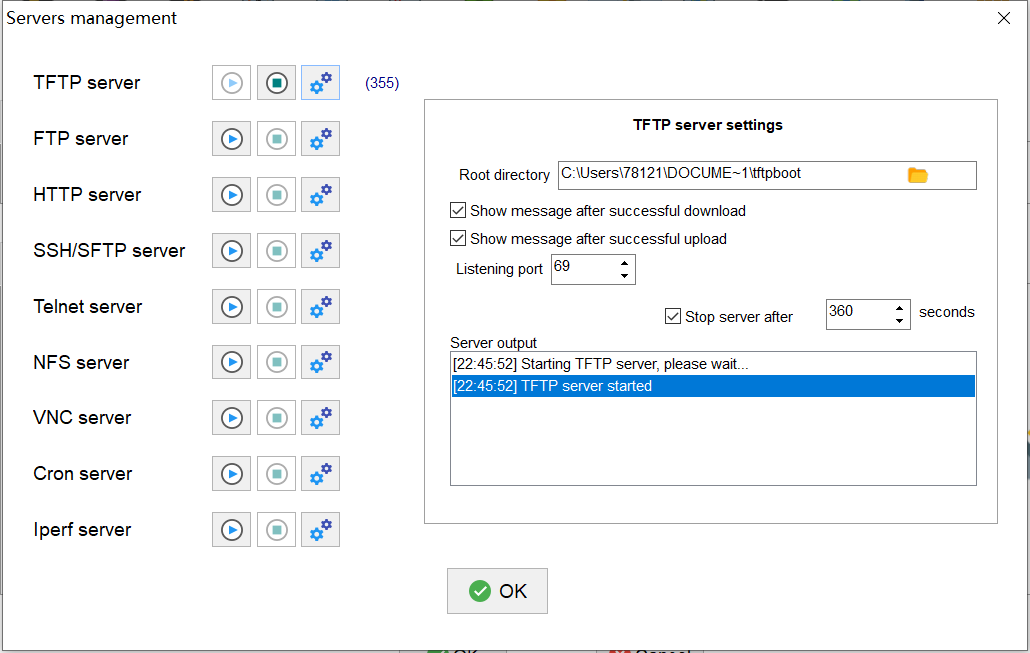
\includegraphics[width=0.8\textwidth]{figures/08-01-mobaXterm教程3.png}
    	\caption{mobaXterm教程3}
    	\label{mobaXterm教程3}
    \end{figure}
    
   \textbf{ 2.linux系统:}这里就来介绍tftp方式从linux主机下载文件到开发板里运行;需要在主机linux系统里安装tftp服务器。在Ubuntu中安装tftp服务器的方法如下:
    
    (1)安装TFTP服务器软件:
   
   \begin{lstlisting}[language=rust]
    sudo apt-get update
    sudo apt-get install tftpd-hpa
   \end{lstlisting}
    
    (2)安装TFTP客户端程序:
    
    \begin{lstlisting}[language=rust]
    sudo apt-get update
    sudo apt-get install tftp
    \end{lstlisting}
    
     (3)配置TFTP服务器:
     
     配置文件通常位于 /etc/default/tftpd-hpa。编辑配置文件并确保以下内容:
     
     \begin{lstlisting}[language=rust]
     TFTP_USERNAME="tftp"
     TFTP_DIRECTORY="/work/tftpboot"  # TFTP服务器的根目录,你可以选择其他目录
     TFTP_ADDRESS="0.0.0.0:69"
     TFTP_OPTIONS="--secure --create"
     \end{lstlisting}
     
     (4)创建TFTP服务器目录并设置权限:
    
    \begin{lstlisting}[language=rust]
    sudo mkdir -p /work/tftpboot  # 创建TFTP服务器的根目录(同(3)中的目录)
    sudo chmod -R 777 /work/tftpboot  # 设置目录权限(同(3)中的目录)
    sudo chown -R nobody:nogroup /work/tftpboot  # 设置目录所有者(同(3)中的目录)
    \end{lstlisting}
    
    (5)启动TFTP服务器服务:
    
     \begin{lstlisting}[language=rust]
    sudo systemctl restart tftpd-hpa  # 启动或重启TFTP服务器服务
    sudo systemctl enable tftpd-hpa   # 设置TFTP服务器随系统启动而自动启动(可选)	
     \end{lstlisting}
    
    (6)验证TFTP服务器是否运行:
    
    可以使用netstat命令检查TFTP服务器是否正在监听端口69:
    
    \begin{lstlisting}[language=rust]
    sudo netstat -anu | grep :69
    \end{lstlisting}
    
    若出现以下结果,则说明tftp服务器正在运行:
    
    \begin{lstlisting}[language=rust]
    udp        0      0 0.0.0.0:69              0.0.0.0:* 
    \end{lstlisting}
    
    (7)测试TFTP服务器:
    
    使用tftp命令测试TFTP服务器是否正常工作。例如,可以尝试从TFTP服务器下载文件或上传文件:
    
    \begin{lstlisting}[language=rust]
	tftp 服务器地址
	tftp> get filename  # 从TFTP服务器下载文件到本地
	tftp> put filename  # 从本地上传文件到TFTP服务器
    \end{lstlisting}
    
    设置TFTP服务器后,确保防火墙允许TFTP流量通过,并根据需要配置相关安全设置。
